% =====================================================================
%  Williamson test case 6 (Rossby--Haurwitz wave) with SFLT stochastic
%  forcing: spatial convergence, solver robustness, energy conservation.
%  Requires \usepackage{booktabs} (and \usepackage{graphicx} for figures).
% =====================================================================

% ---------------------------------------------------------------------
%  Table 1: spatial convergence of the stochastic scheme
% ---------------------------------------------------------------------
\begin{table}[htbp]
  \centering
  \begin{tabular}{c c c c c c}
    \toprule
    ref & $h$ (km) & $\|u-u_{\mathrm{ref}}\|_{L^2}$ & rate$_u$
        & $\|D-D_{\mathrm{ref}}\|_{L^2}$ & rate$_D$ \\
    \midrule
    2 & 1785.5 & $1.27\times10^{7}$ & --   & $5.45\times10^{8}$ & --   \\
    3 &  892.8 & $1.72\times10^{6}$ & 2.89 & $1.38\times10^{8}$ & 1.98 \\
    4 &  446.4 & $2.73\times10^{5}$ & 2.66 & $3.36\times10^{7}$ & 2.04 \\
    \bottomrule
  \end{tabular}
  \caption{Spatial (strong) convergence of the SFLT stochastic, energy-conserving
    scheme for Williamson test case~6, BDM$_2$/DG$_1$, cPG($P_1$) in time,
    $t = 2$\,days. The same noise realization is shared across meshes by
    cross-mesh interpolation, and a fine mesh (refinement level~5) serves as the
    numerical reference; errors are area-weighted $L^2$ norms averaged over three
    seeds. The correlation length is set to $\lambda = 6\times10^{6}$\,m so the
    noise is resolved on every mesh ($\lambda/h > 3$ at the coarsest level). The
    depth converges at the expected second order; the velocity is
    super-convergent ($\sim\!2.7$), matching the deterministic Williamson~6
    spatial rates -- i.e.\ adding resolved transport noise does not degrade the
    spatial accuracy of the compatible finite-element discretisation.}
  \label{tab:w6-sflt-spatial}
\end{table}

% ---------------------------------------------------------------------
%  Table 2: solver robustness and energy conservation vs mesh
% ---------------------------------------------------------------------
\begin{table}[htbp]
  \centering
  \begin{tabular}{c c c c}
    \toprule
    ref & $h$ (km) & avg.\ linear iters / step & $|(E-E_0)/E_0|$ \\
    \midrule
    2 & 1785.5 &  9.82 & $2.0\times10^{-8}$  \\
    3 &  892.8 & 10.10 & $1.6\times10^{-9}$  \\
    4 &  446.4 & 11.00 & $9.9\times10^{-11}$ \\
    5 &  223.2 & 12.00 & $6.0\times10^{-12}$ \\
    \bottomrule
  \end{tabular}
  \caption{Solver robustness and energy conservation of the SFLT scheme for
    Williamson test case~6, BDM$_2$/DG$_1$, cPG($P_1$), $\Delta t$ fixed by
    $\texttt{nsteps}=400$ over $2$\,days. The average number of Krylov (GMRES with
    a star-patch additive-Schwarz preconditioner) iterations per timestep is
    essentially mesh-independent, growing only from $9.8$ to $12.0$ across an
    eight-fold refinement \emph{with the stochastic forcing active} -- the noise
    does not degrade solver performance. The relative energy drift (final value,
    seed~1) is at solver/round-off level and tightens with resolution, confirming
    that the scheme remains discretely energy-conserving in the presence of
    transport noise.}
  \label{tab:w6-sflt-robust}
\end{table}

% ---------------------------------------------------------------------
%  Table 3: temporal (strong) convergence -- weak vs strong noise
% ---------------------------------------------------------------------
\begin{table}[htbp]
  \centering
  \begin{tabular}{c c c c c c}
    \toprule
    \texttt{nsteps} & $\Delta t$ (s) & $\|u-u_{\mathrm{ref}}\|_{L^2}$ & rate$_u$
        & $\|D-D_{\mathrm{ref}}\|_{L^2}$ & rate$_D$ \\
    \midrule
    200  & 864 & $6.19\times10^{7}$ & --   & $1.37\times10^{9}$ & --   \\
    400  & 432 & $4.46\times10^{7}$ & 0.47 & $1.05\times10^{9}$ & 0.39 \\
    800  & 216 & $2.75\times10^{7}$ & 0.70 & $6.77\times10^{8}$ & 0.63 \\
    1600 & 108 & $1.43\times10^{7}$ & 0.94 & $3.38\times10^{8}$ & 1.00 \\
    \bottomrule
  \end{tabular}
  \caption{Temporal (strong) convergence of the SFLT stochastic scheme for
    Williamson test case~6 on a fixed mesh (refinement level~4), cPG($P_1$) in
    time, $t = 2$\,days. All timestep sequences share a single Brownian path: the
    finest run ($\texttt{nsteps}=6400$) saves the noise increments $\mathrm{d}W$
    and the coarser runs sum them, so every $\Delta t$ integrates the \emph{same}
    realization; the $\texttt{nsteps}=6400$ run is the reference and is a factor
    of four or more finer than every tabulated step, so all rates are
    uncontaminated. Errors are area-weighted $L^2$ norms averaged over two seeds
    (seed scatter $\lesssim 0.5\%$). At physical noise amplitude
    ($u_{\mathrm{noise}}/u \approx 0.2$, correlation length $\lambda = 10^{6}$\,m)
    the stochastic $\mathcal{O}(\Delta t^{1/2})$ transport term dominates the
    error and the scheme exhibits the expected \emph{strong order between $0.5$
    and $1.0$} of Stratonovich transport noise (the measured rate rises from
    $\approx 0.5$ at coarse $\Delta t$ towards $\approx 1.0$ as $\Delta t$ is
    refined).
    %
    This contrasts sharply with the \emph{weak/resolved} noise regime
    ($\lambda = 6\times10^{6}$\,m, $u_{\mathrm{noise}}/u \approx 0.003$), where
    the deterministic part of the error dominates and the scheme recovers its
    full deterministic order ($\approx 2$, the cPG($P_1$) rate). The observed
    temporal order is thus set by which contribution -- stochastic or
    deterministic -- dominates at the given noise amplitude.}
  \label{tab:w6-sflt-temporal}
\end{table}

% ---------------------------------------------------------------------
%  Diagnostic figures (require \usepackage{graphicx})
%  Upload w6_energy_errors_SFLT.png and w6_div_norms_SFLT.png to Overleaf.
% ---------------------------------------------------------------------
\begin{figure}[htbp]
  \centering
  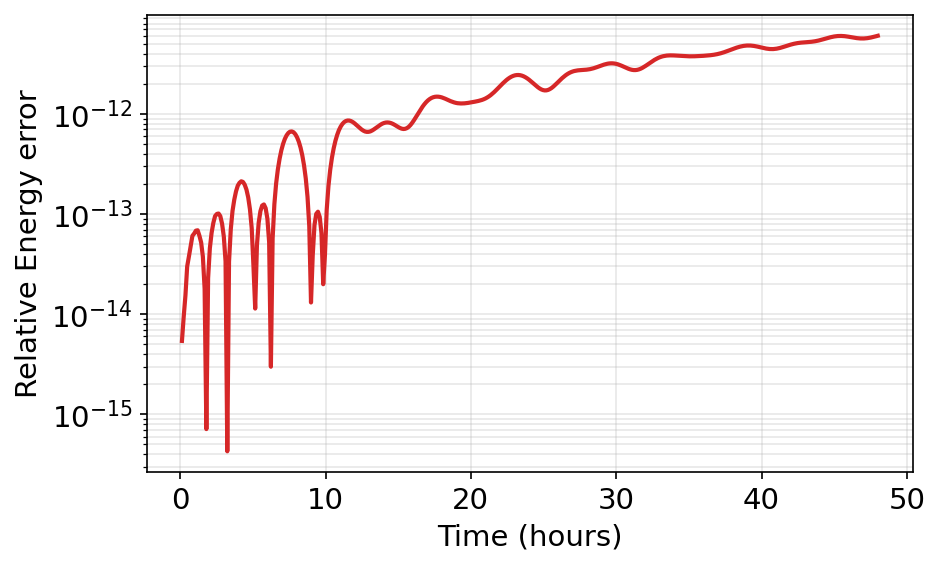
\includegraphics[width=0.8\textwidth]{w6_energy_errors_SFLT.png}
  \caption{Relative energy drift $|(E-E_0)/E_0|$ versus time for Williamson test
    case~6 \emph{with} SFLT stochastic forcing, BDM$_2$/DG$_1$ on refinement
    level~5, cPG($P_1$), $\Delta t = 432$\,s over two days. The energy exhibits
    only a slow systematic drift of magnitude $\lesssim 6\times10^{-12}$ (a
    per-step change $\sim\!6\times10^{-15}$, at the iterative-solver/round-off
    level: the cPG($P_1$)/implicit-midpoint scheme conserves the quadratic energy
    exactly only when the algebraic system is solved exactly). The stochastic
    transport term contributes no net energy -- it enters as an energy-conserving
    (Stratonovich, divergence-free) perturbation rather than a spurious source or
    sink -- so the discrete energy-conservation property of the scheme is
    preserved in the presence of noise.}
  \label{fig:w6-sflt-energy}
\end{figure}

\begin{figure}[htbp]
  \centering
  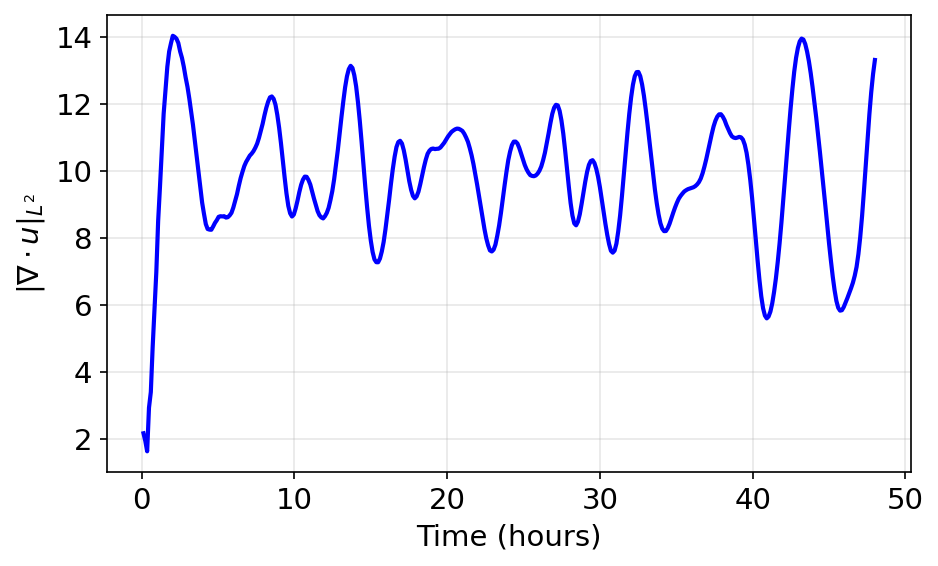
\includegraphics[width=0.8\textwidth]{w6_div_norms_SFLT.png}
  \caption{Velocity divergence $\|\nabla\cdot u\|_{L^2}$ versus time for Williamson
    test case~6 with SFLT stochastic forcing, BDM$_2$/DG$_1$ on refinement
    level~5 with $\Delta t = 432$\,s. The stochastic velocity increment is
    $u_{\mathrm{noise}} = \nabla^{\perp}\psi_{\mathrm{noise}}$, i.e.\
    divergence-free by construction, so the noise injects no spurious divergence:
    the $\|\nabla\cdot u\|$ trace remains bounded and is statistically
    indistinguishable from the deterministic run (cf.\ Fig.~\ref{fig:w6-div}).}
  \label{fig:w6-sflt-div}
\end{figure}
